\section{Entwurf eines Vordergrund-Extraktors}
\label{chap:entwurf}

In diesem Kapitel wird der nötige, theoretische Hintergrund herausgearbeitet und unser Entwurf gemäß den Anforderungen vorgestellt.
Es wird das Konzept der Hidden-Markov-Modelle (HMM) und der Diskreten Kosinustransformation(DCT) erläutert und deren Verknüpfung eingeführt.
%TODO: Kommentar unklar: "mit fehlenden werten pro pixel ..."


\subsection{Anforderungsanalyse}
\label{sec:anforderungsanalyse}

Die funktionalen Anforderungen an einen Vordergrund-Extraktor sind bereits in der Aufgabenbeschreibung (\ref{sec:aufgabenbeschreibung} ausgeführt:
Es soll demonstriert werden, dass HMM zur Trennung von Vordergrund und Hintergrund bei stark heterogenen Hintergründen geeignet sind, wie in Abbildung \ref{fig:foreground} dargestellt.
\begin{figure}[H]
	\centering
	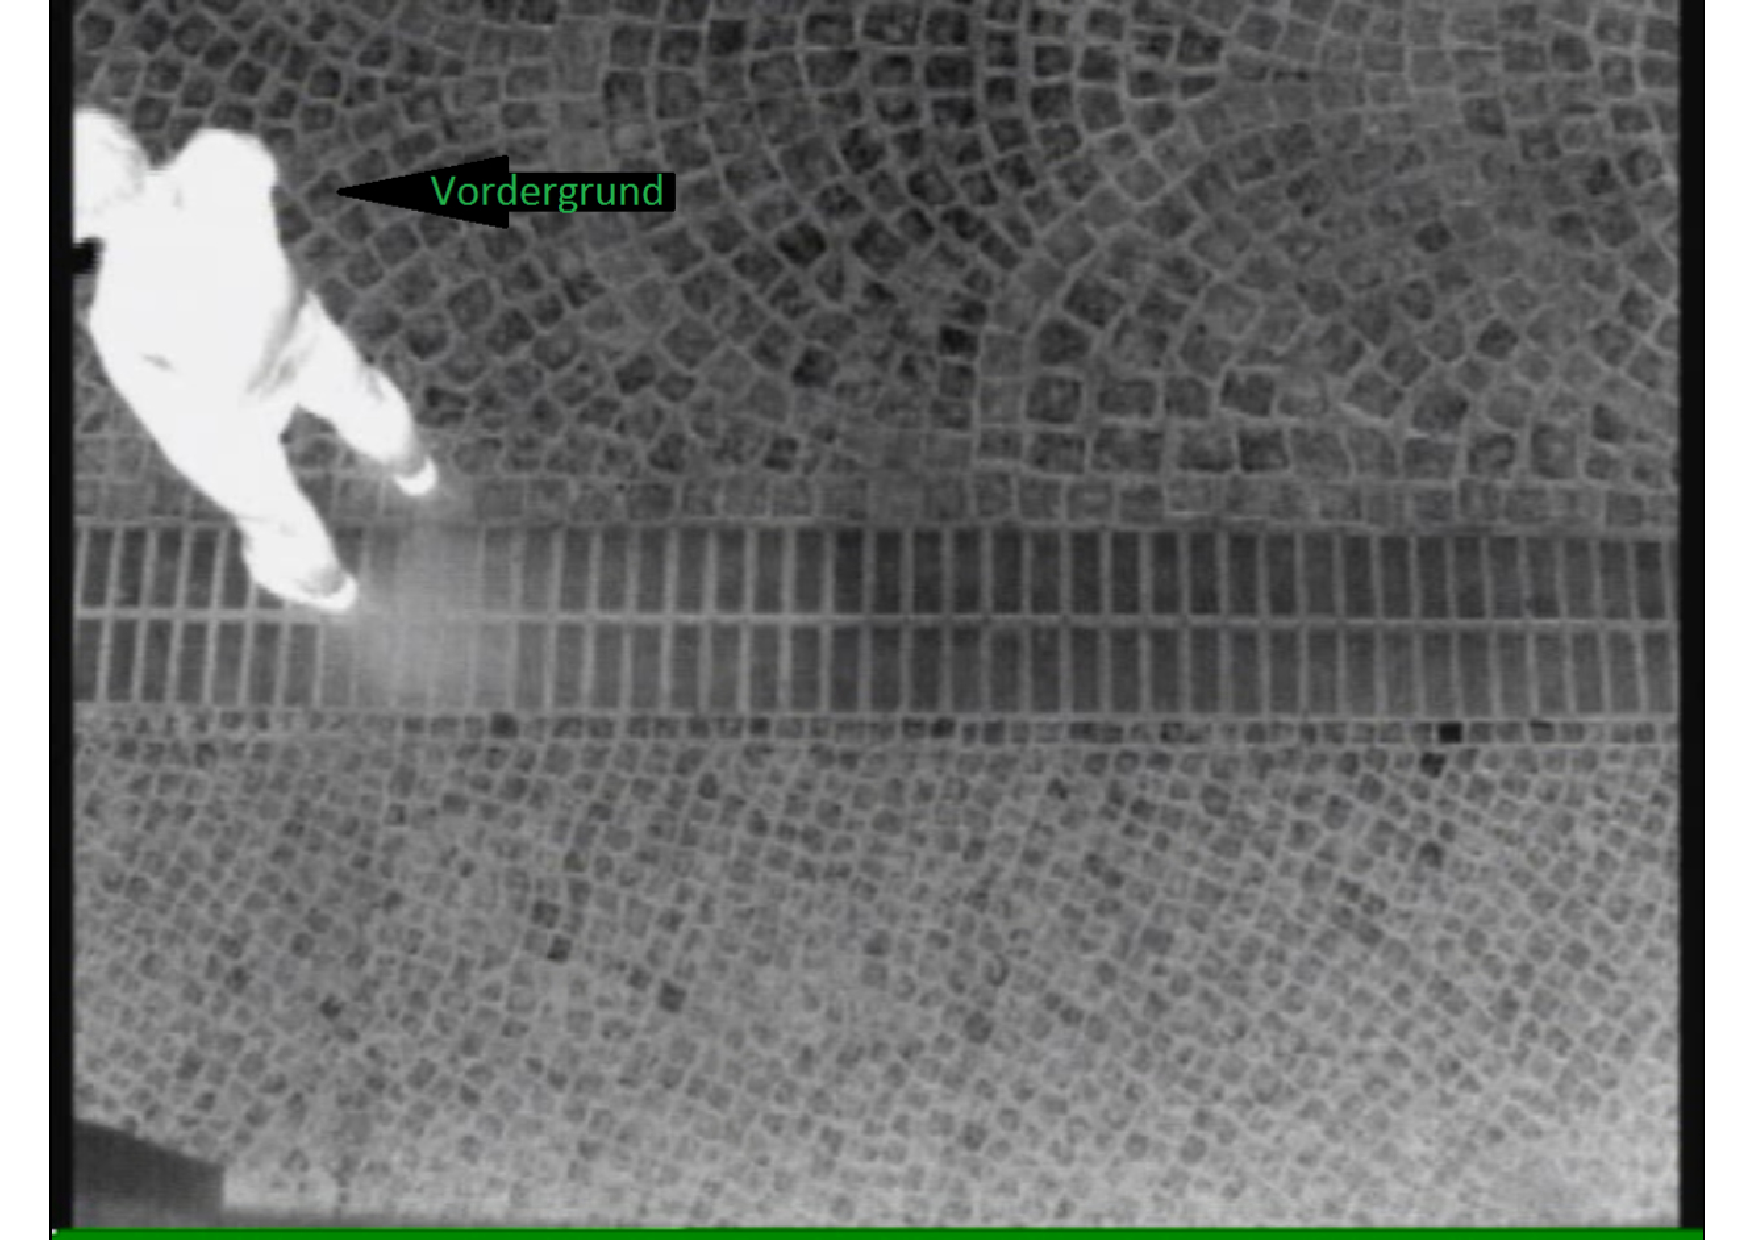
\includegraphics[width=1\textwidth]{bilder/01_foreground.pdf}
	\caption{Kamerabild, Vordergrund ist markiert}
	\label{fig:foreground}
\end{figure}
Die nichtfunktionalen Anforderungen umfassen vor allem eine einfache Benutzbarkeit durch Automatisierung.
Der Ressourcenbedarf soll möglichst gering sein - ein Video wird für gewöhnlich mit 25 Frames pro Sekunde aufgezeichnet, im Idealfall ist eine optimale Analyse jedes einzelnen Frames in Echtzeit möglich.
%Hierbei ist zu beachten, dass eine hohe Korrektheit zu erzielen ist, das heißt, dass die Ergebnisse fehlerfrei sein müssen.
Allerdings ist zu berücksichtigen, dass eine möglichst hohe Korrektheit wichtiger ist, als eine Analyse in Echtzeit. Falls nötig können auch Bilder ausgelassen werden.
%Eine Flexibilität bezüglich unterschiedlicher Videotypen ist gewünscht, also die Unterstützung von variierenden Videoauflösungen et cetera.
Die Analyse sollte jedoch unabhängig von den Parametern des verwendeten Videomaterials wie beispielsweise unterschiedliche Videoformate oder Auflösungen statt finden.


\subsection{Hidden-Markov-Modelle}
\label{sec:hiddenmarkovmodel}

Die Markov Modelle stammen aus der Wahrscheinlichkeitstheorie und entsprechen einem stochastischem Zustandsautomaten, bei dem die Zustandswechsel gemäß einer Wahrscheinlichkeit statt finden und nicht abhängig von der Vergangenheit sind, sondern nur von dem aktuellen Zustand.
%TODO: Kommentar: etwas salopp formuliert: sollte also nochmal überarbeitet werden.
Bei den HMM\cite{Stamp04arevealing} können jene Zustände nicht beobachtet werden, sondern nur die Beobachtungen/Ausgaben, welche während dieses Zustandes auftreten, sie werden Emissionen genannt.
Die Zustandsübergangswahrscheinlich- keiten sind in den HMM somit nicht die einzigen Parameter, die Emissionswahrscheinlichkeiten bilden die zweiten Parameter.\\
Formal definiert ist ein HMM ein 5er-Tupel $\lambda= (S, V, A, B, \Pi)$ mit:
\begin{itemize}
 \item $S = {s_1,..., s_n}$ sei die Menge aller Zustände
 \item $V = {v_1,..., v_m}$ das Alphabet der möglichen Emissionen
 \item $A \in \mathbb{R}^{n \times n}$ sei eine Übergangsmatrix zwischen den Zuständen, $a_{ij}$ entspricht der Wahrscheinlichkeit des Übergangs von Zustand $s_i$ in Zustand $s_j$
 \item $B \in \mathbb{R}^{n\times m}$ sei eine Beobachtungsmatrix, wobei $b_i(v_j)$ die Wahrscheinlihkeit angibt, im Zustand $s_i$ die Beobachtung (Emission) $v_j$ zu sehen
 \item $\Pi \in R^n$ die Initialverteilung, $\Pi_i$ sei die Wahrscheinlichkeit, dass $s_i$ der Startzustand ist
\end{itemize}
Ein HMM heißt zeitinvariant, wenn sich die Übergangs- und Emissionswahrscheinlichkeiten nicht mit der Zeit ändern.\\
HMM werden zunehmend in der Literatur zur Sprach-, Schrift und Mustererkennung \cite{Gales:2007:AHM:1373536.1373537}\cite{Yang1995161} verwendet, da sie mit den probabilistischen Übergängen die Prozesse der echten Welt besser widerspiegeln als deterministische Definitionen, zu dem können die Parameter durch Lernalgorithmen automatisiert bestimmt werden.
 siehe hierzu Kapitel 2.5.
\begin{figure}[H]
	\centering
	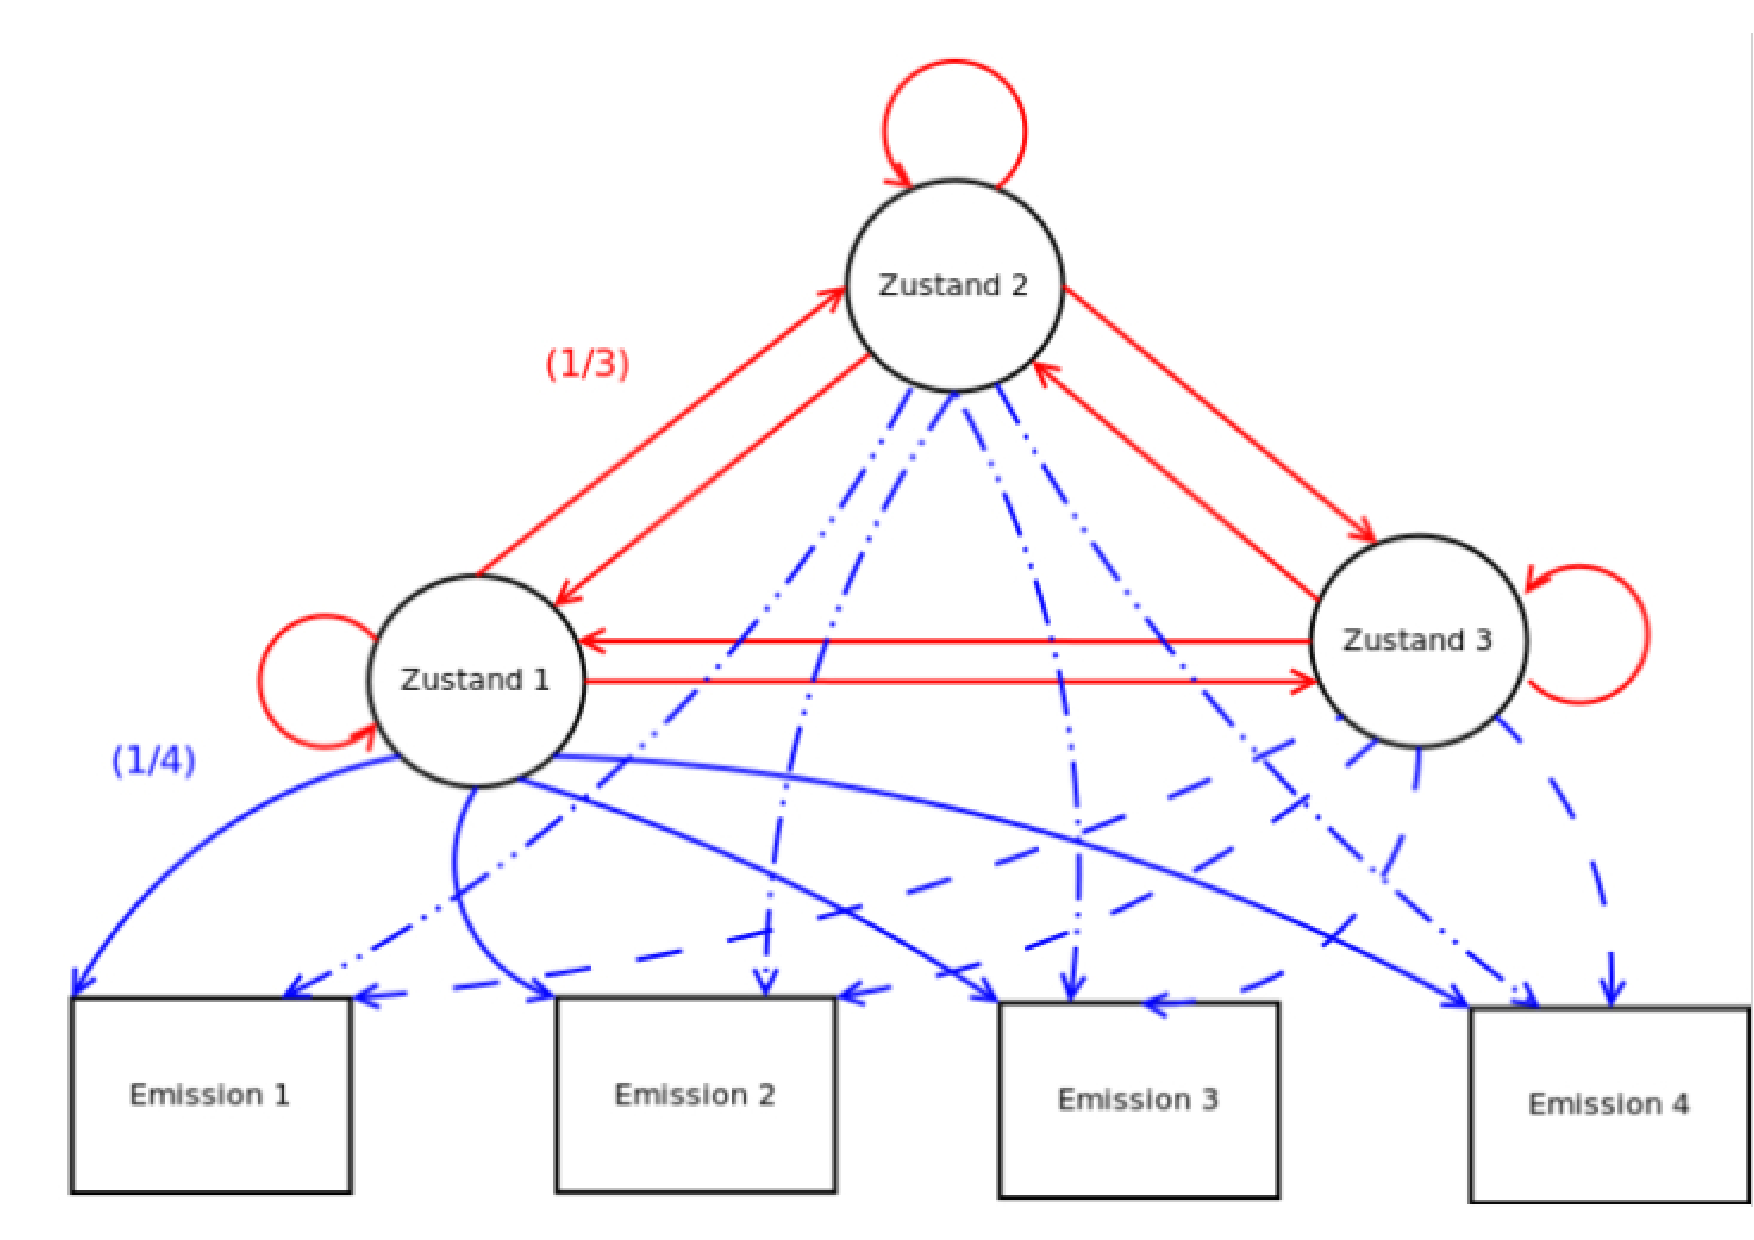
\includegraphics[width=1\textwidth]{bilder/02_hmm.pdf}
	\caption{Beispiel für ein HMM}
	\label{fig:hmm}
\end{figure}
Abbildung \ref{fig:hmm} zeigt ein HMM mit 3 Zuständen und 4 Emissionen, wobei der Übergang aus jedem Zustand zu jedem Zustand und zusätzlich in jedem Zustand jede Emission möglich ist.
In diesem Beispiel liegt eine Gleichverteilung vor, Übergänge zwischen Zuständen haben stets die Wahrscheinlichkeit $1/3$, die Emissionen haben stets eine Wahrscheinlichkeit von $1/4$.
Beschriftung der Kanten aus Übersichtsgründen nicht dargestellt.
%TODO: Bedeutung von Beispiel/Grafik, wieso gleichverteilt, Quelle?

\subsection{Standartalgorithmen von HMMs}
\label{sec:standartalgorithmenHMM}
%TODO: Alexandras Vorschlag: Gängige Problemstellungen

Für die HMM wurden bereits viele Algorithmen entwickelt, welche Standardprobleme lösen.
Die zwei häufigsten Problemstellungen bei HMMs sind das Lernproblem und das Evaluations-/Decodingproblem.
\begin{enumerate}
	\item Das Lernproblem bezieht sich auf die Problematik ein HMM so zu trainieren, dass man im Folgenden das HMM dafür nutzen kann, Aussagen über die wahrscheinlichsten Folgezustände zu treffen.
Gelöst wird dieses Problem durch den Baum-Welch Algorithmus, welcher dazu verwendet wird, unbekannte Parameter, genauer die Übergangs- und Emiossionswahrscheinlichkeiten eines HMM, zu bestimmen.
 Hierbei handelt es sich um einen erwartungsmaximierenden Algorithmus, welcher anhand von übergebenen Trainingssequenzen die Maximum-Likelihood-Schätzwerte berechnet.
 Die initialen Werte eines HMMs müssen geschätzt werden, hier wird für gewöhnlich eine Gleichverteilung angenommen, dass heißt das jeder Übergang und jede Emission in einem Zustand gleich wahrscheinlich sind.
	\item Das Evaluations-/Decodingproblem bezieht sich auf die Problemaik aus den verschieden Wahrscheinlichkeiten Aussagen über die Folgezustände oder aber über die Wahrscheinlichkeit bestimmter Zustandsketten zu treffen.
Es wird durch den Forward-Algorithmus beziehungsweise den eng verwandten Viterbi-Algorithmus gelöst.
Gegeben sei eine Chronik an k-letzten Emissionen, was ist die Wahrscheinlichkeit für eine bestimme Emission? Und ferner, was ist die wahrscheinlichste Emission? Der Viterbi-Algorithmus berechnet zur Beantwortung dieser Frage die wahrscheinlichste Zustandssequenz, also eine Sequenz die die Wahrscheinlichkeit der übergebenen Emissionssequenz maximiert, und kann anhand des letzten Zustandes dieser Sequenz das Problem lösen.
Der Forward-Algorithmus ist ein Algorithmus aus der dynamischen Programmierung und optimiert im Gegensatz zum Viterbi nicht rückwirkend die gesamte Zustandssequenz neu, sondern berechnet den aktuell wahrscheinlichsten Zustand auf Basis der zuvor berechneten Zustände und hängt diesen an.
Somit ist der Forward Algorithmus zur Laufzeit grundsätzlich schneller, jedoch nicht so genau wie der Viterbi-Algorithmus.
 \end{enumerate}


\subsection{Diskrete Kosinustransformation}
\label{sec:dct}

Die Diskrete Kosinustransformation (DCT)\cite{Khayam03thediscrete} ist ein Verfahren, welches zur verlustbehafteten Kompression von Daten verwendet wird, wobei die bekannteste Anwendung das Dateiformat JPEG ist.
Ähnlich zu der diskreten Fourier Transformation wird eine Information mittels Frequenzen repräsentiert, wobei wie der Name bereits nahe legt nur Kosiunusfunktionen verwendet werden.


Es existieren mehrere Varianten der DCT.
Wird jedoch die DCT auf Bildinformationen angewandt, speziell bei der JPEG-Kompression, so wird die zwei-dimensionale Typ II DCT verwendet, welche die gängiste Variante ist.
%TODO: Anmerkung: wieso ist DCT-II die gängigste Variante?
Die DCT erhält eine $n \times  n$ Matrix und gibt eine Matrix der selben Größe zürück, wobei im JPEG-Standard $8 \times 8$ Pixel Matrizen betrachtet werden.
Hierbei wird das Element $[1,1]$ als DC-Wert bezeichnet und bildet den Durchschnittswert der Farben der betrachteten Matrix; die restlichen 63 Werte der Matrix sind ein Offset zu dem DC-Wert und kodieren somit den Unterschied zum DC-Wert innerhalb der Matrix.
Diese Werte werden als AC-Werte bezeichnet.\\
Formal definiert ist die DCT eine lineare, invertierbare Funktion $f : \mathbb{R}^n \rightarrow \mathbb{R}^n$, welche $N$ reellwertige Werte aus $x[n]$ in $N$ reellwertige Werte nach $X[n]$ überführt:\\

\begin{centering}
$X_k = \sum\limits_{n=0\rightarrow N-1} x_n \cos [\frac{\Pi}{N} + (n + \frac{1}{2}) k ]$ mit $k = 0,..., N-1$\\
\end{centering}

Abbildung \ref{fig:dct} zeigt das Ergebnis nach der Anwendung der DCT mit Einfärben der gesamten Blöcke in die jeweils berechneten DC-Werte.
\begin{figure}[H]
	\centering
	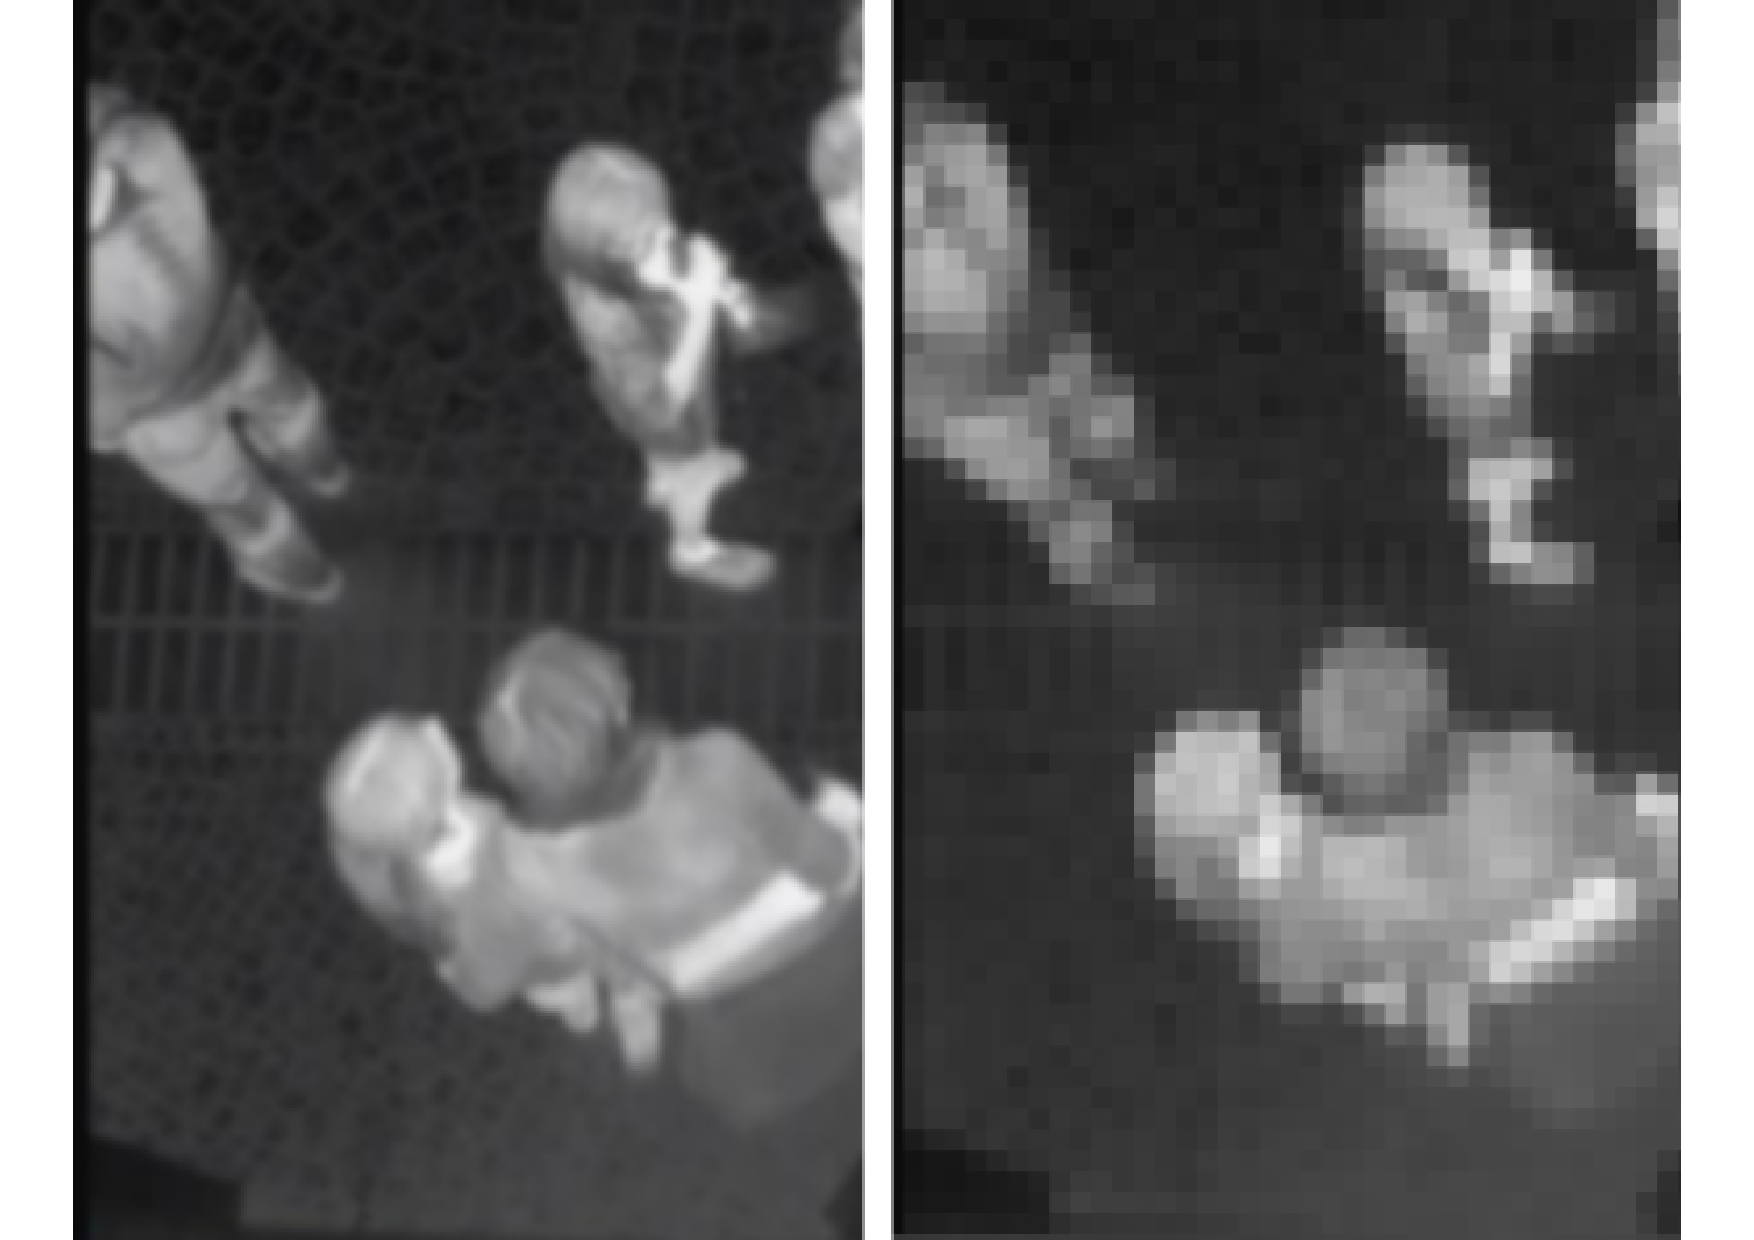
\includegraphics[width=1\textwidth]{bilder/03_dct_dc-only.pdf}
\caption{Links: Originalbild, rechts: Bild nach Anwendung der DCT blockweise nach DC-Wert eingefärbt}
	\label{fig:dct}
\end{figure}

\subsection{Modellierung eines Eingabealphabets}
\label{sec:modellierungeingabealphabet}
In unserem Projekt sollen HMM benutzt werden, um eine Entscheidung zu treffen, ob ein Bildbereich zum Vorder- oder zum Hintergrund gehört.
Nach dem das generelle Konzept von HMM in Kapitel \ref{sec:hiddenmarkovmodel} vorgestellt wurde, fehlt jedoch noch die Definition, wie eine Emission aussieht.
Das Alphabet der Emissionen wird als Eingabealphabet bezeichnet, da mit dessen Hilfe das System beschrieben werden kann.
Hierbei ist zu beachten, dass das Eingabealphabet endlich und diskret sein muss.
Zusätzlich sollte das Eingabealphabet aus möglichst wenigen, aussagekräftigen Symbolen bestehen.
Die Kodierung, also die Zuordnung von Daten zu bestimmten Emissionen,  eines Eingabealphabets gehört daher in unserem Fall zu der Kernleistung bei der Verwendung von HMM.\\
Die im Kapitel \ref{sec:standartalgorithmenHMM} vorgestellte DCT wird von uns verwendet, um ein Eingabealphabet zu erzeugen, wobei wir die DCT auf fest definierte Bereiche anwenden.
Wir übernehmen die aus der Bildkompression üblichen 8 x 8 Pixelblöcke zur Einteilung des vorliegenden Bildes, da wir dieses als optimalen Kompromiss zwischen einer zu hohen und niedrigen Granularität ansehen: kleinere Betrachtungen, so zum Beispiel pixelbasierte Verfahren, wären deutlich rechenintensiver und anfälliger auf Bildrauschen und würden daher keine akkuraten Rückschlüsse bei Veränderungen des Pixelwertes ermöglichen.
Bei größeren Betrachtungen wären relevante Veränderungen deutlich schwerer wahrzunehmen, speziell im DC-Wert, da dieser stets den Mittelwert aller Subpixel der Matrix darstellt.

\subsubsection{DC-Wert}
\label{sec:dc-wert}

Da Bildaufnahmen von Mittelinfrarot-Kameras stets schwarzweiß sind (und warme Bereiche heller dargestellt werden als kühle) besitzt ein Pixel genau einen Informationskanal mit einem Grauwert zwischen 0 (schwarz) bis 255 (weiß).
Der DC-Wert liegt somit als Mittelwert ebenso in diesem Intervall.
Dieser Bereich ist zu groß um als Eingabealphabet für das HMM dienen zu können, da zum Beispiel der Übergang von einem Grauwert von 230 auf 235 nicht aussagekräftig ist, da es sich hierbei um Rauschen oder aber eine Neukalibrierung der Kamera, die sich ja stets auf die gesamte $8 \times 8$ Matrix auswirkt, halten kann.\\

Wir nehmen jedoch eine Dreiteilung des Wärmespektrums an, einen kühlen Hintergrund, warmen Vordergrund und ein mittelwarmen Bereich.
Diese Dreiteilung ergibt sich daraus, dass es sehr wahrscheinlich ist, dass sehr helle Bereiche zum Vordergrund und sehr dunkle Bereiche zum Hintergrund gehören.
Bei dem größten Bereich, der aus verschiedenen Grauwerten besteht, ist eine einfache Zuordnung allerdings nicht möglich. Mehr Teile machen hingegen auch keinen Sinn, da diese dann nur Zuordnungen wie "wahrscheinlich Vordergrund" oder "wahrscheinlich Hintergrund" zuliessen, diese Wahrscheinlichkeiten aber durch das HMM bereits mit einem unsicheren Teil abgebildet werden.
Histogramm-basierte Analysen der DC-Werte über mehrere unterschiedliche Videosequenzen über alle Pixelblöcke genormt bestätigen diese Annahme und manifestieren 3 Cluster, die wir vereinfacht Cluster schwarz, Cluster grau und Cluster weiß nennen - der Darstellungsfarbe des Wärmespektrums entsprechend.
Die Grenzen dieser Cluster sind abhängig von jedem Video und dem betrachteten Umfeld, denn die insbesondere die Kälte (und damit die Farbe) des Hintergrundes kann sich bei den jeweiligen Videos stark unterscheiden.\\
Wir bilden auf Basis dieser Erkenntnis die ersten 3 Symbole, wobei, wenn der DC-Wert eines Blockes in das Intervall eines Clusters fällt, wir die entsprechende Beobachtung erstellen:
\begin{itemize}
	\item DC-Wert im Intervall Cluster schwarz $\rightarrow$ Beobachtung: DC\_BLACK
	\item DC-Wert im Intervall Cluster grau$\rightarrow$ Beobachtung: DC\_GREY
	\item DC-Wert im Intervall Cluster weiß $\rightarrow$ Beobachtung DC\_WHITE
\end{itemize}
Abbildung \ref{fig:histogram}Bild zeigt eine exemplarische Einteilung in die drei Cluster.
Die X-Achse beschreibt dabei den Grauwert, die Y-Achse die Anzahl Blöcke eines bestimmten Grauwerts.
Für die Erstellung des Histograms wurden sämtliche Grauwerte aller Blöcke eines Testvideos über die gesamte Länge des Videos erfasst.
\begin{figure}[H]
	\centering
	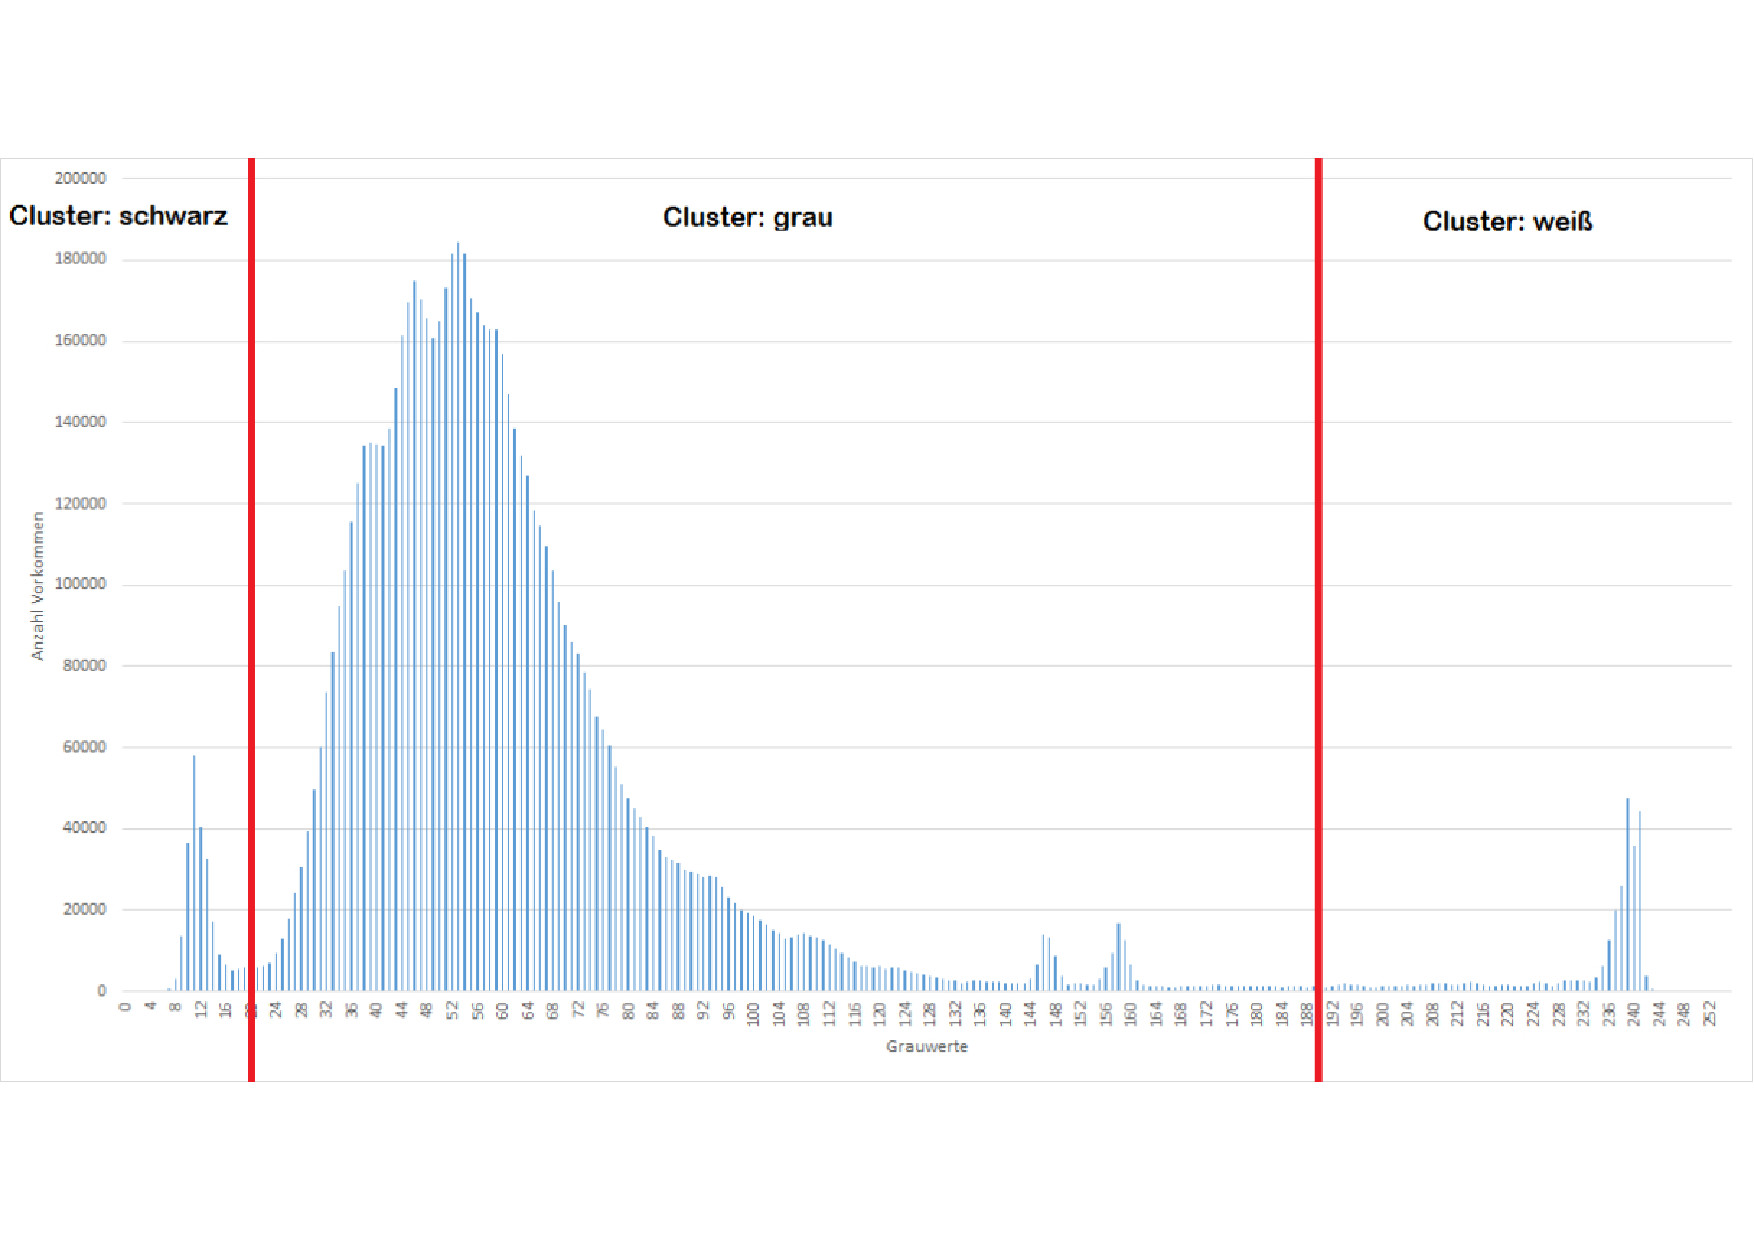
\includegraphics[trim=0cm 3cm 0cm 3cm, clip=true,width=1\textwidth]{bilder/04_histogram_cluster.pdf}
	\caption{Histogramm über alle DC-Werte aller Blöcke einer Videosequenz, Clustergrenzen rot}
	\label{fig:histogram}
\end{figure}

\subsubsection{AC-Wert}
\label{sec:ac-wert}

Die bei der Anwendung der DCT entstehende 8 x 8 Matrix enthält 63 AC-Werte, diese bilden demnach den Großteil der in der Matrix kodierten Informationen; die Integration dieser Werte in das Eingabealphabet ist aufgrund der hohen Informationsdichte essenziell.\\
Eine Histogramm-basierte Betrachtung der AC-Werte analog zu der Betrachtung der DC-Werte ist nicht zielführend, da es sich hierbei um Offsets handelt, welche demnach im Histogramm ein Maximum um den Nullwert bilden.
Wir erkennen jedoch, das Menschen aufgrund ihrer warmen Austrahlung eine starke Kante zu dem Hintergrund bilden, läuft demnach ein Mensch durch einen Block, müsste eine deutliche Abweichung einiger AC-Werte zum DC-Wert entstehen.
Eine Block-basierte Analyse bestätigt diese Annahme, die Standardabweichung (STD) der AC-Werte bezüglich des DC-Wertes steigt deutlich an, falls eine Person sich im Block befindet beziehungsweise durch diesen hindurch läuft.\\
Abbildung \ref{fig:ac_over_time} stellt auf der X-Achse den Zeitverlauf in Frames und auf der Y-Achse den Wert der Standardabweichung für den betrachteten Bock; es lässt sich feststellen, dass die Kurve der Standabweichung stark ausschlägt, falls eine Person durch den Block läuft.\\
\begin{figure}[H]
	\centering
	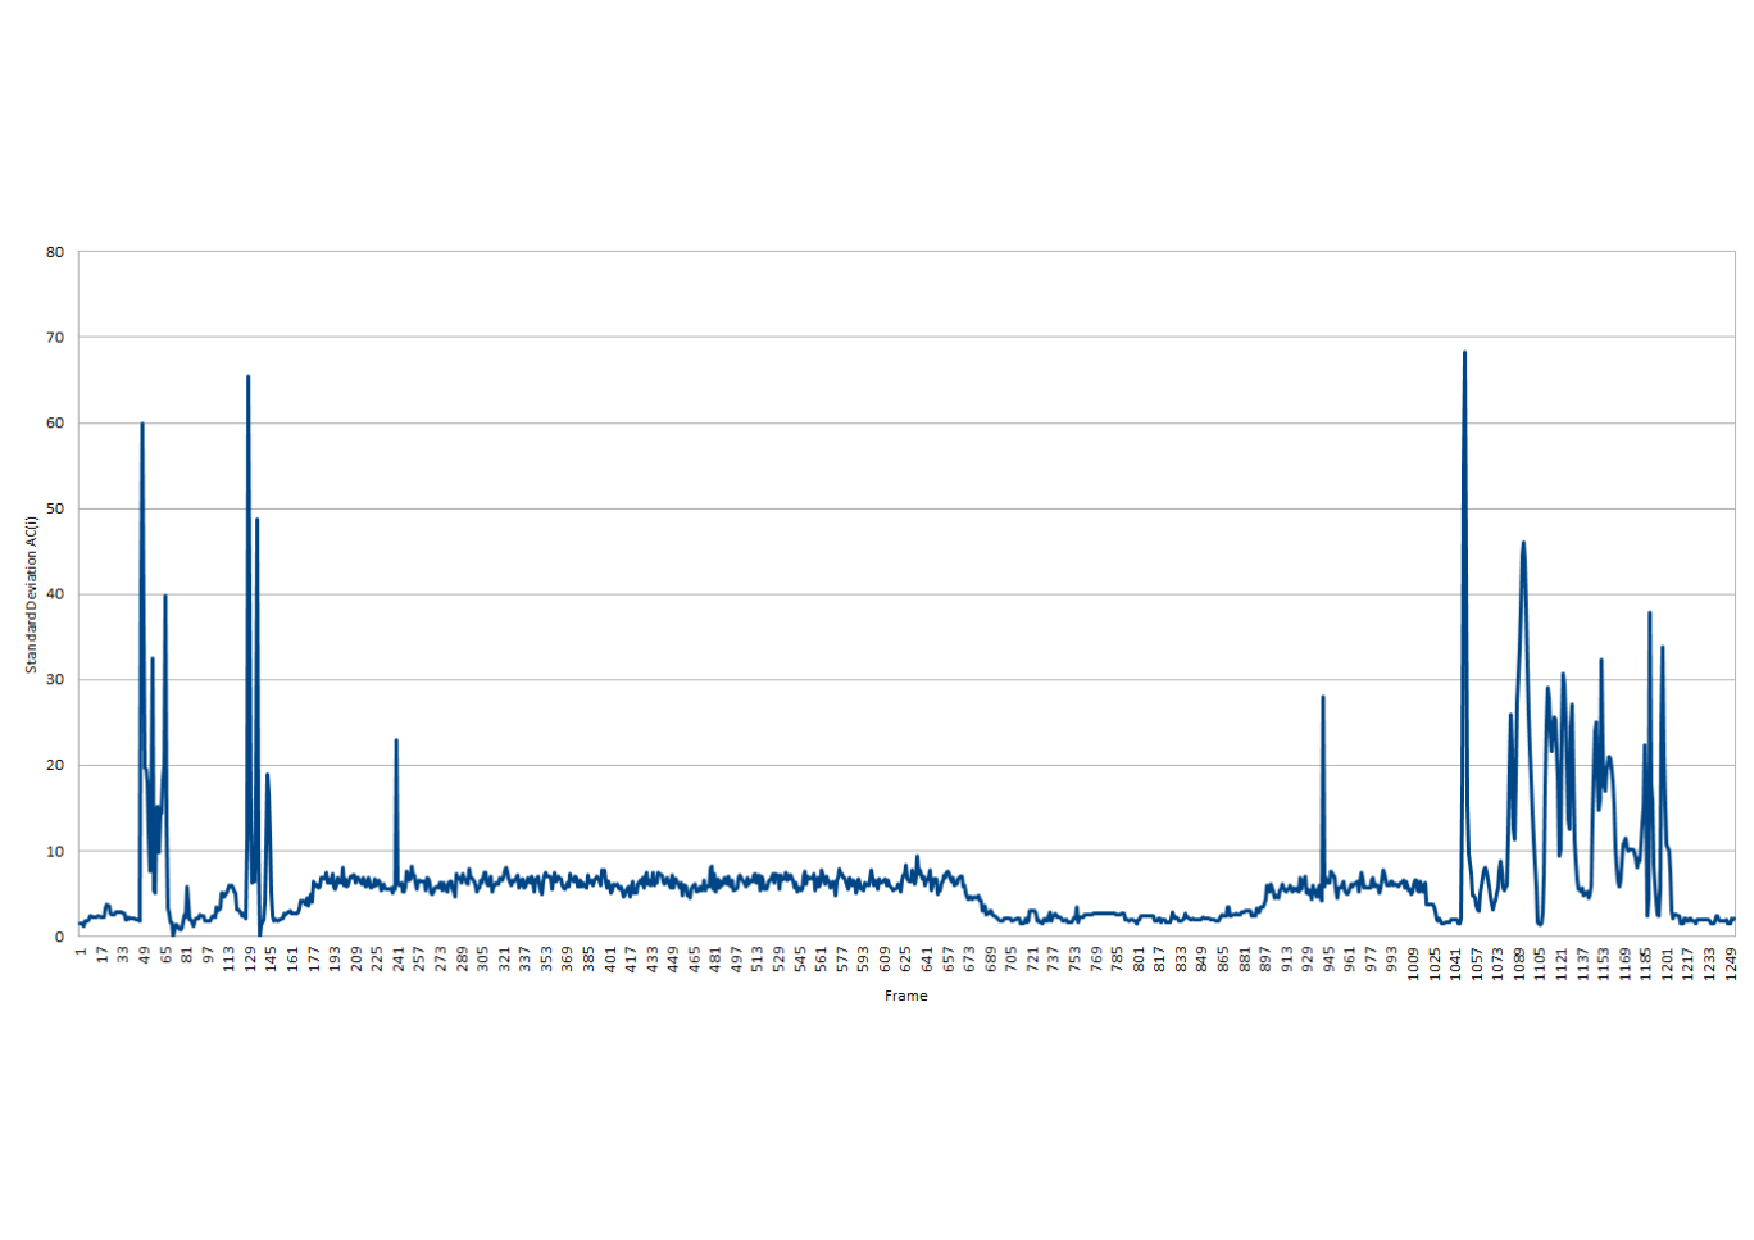
\includegraphics[trim=0cm 4.5cm 0cm 4cm, clip=true,width=1\textwidth]{bilder/05_AC_over_time.pdf}
	\caption{Standartabweichung der AC-Werte eines diskreten Blocks über der Zeit}
	\label{fig:ac_over_time}
\end{figure}
Anhand von empirischen Tests lässt sich eine Grenze ermitteln.
Falls die Standardabweichung diese übersteigt, betritt oder verlässt mit hoher Wahrscheinlichkeit eine Person den betrachteten Block.
In dem vorgestellten Beispiel liegt dieser bei 25.\\
Zusätzlich ist zu beachten, dass die Standardabweichung von wenigen, aber extremen statistischen Ausreißern kaum beeinflusst wird, diese Situation liegt  jedoch während der Erkennung von Menschen vor, insbesondere bei Personen, die Kleidung tragen, welche die Wärmeabgabe der Person dämmt, und dennoch einige freiliegende Körperteile sichtbar sind.
In diesem Fall ist der Großteil der AC-Werte relativ klein und der DC-Wert des betrachteten Blockes für gewöhnlich innerhalb des grauen Intervalls.
Um in diesen Situationen den Vordergrund besser zu erkennen, prüfen wir mithilfe eines selbstdefinierten Verfahrens outliers() ob stark-positive (warme) Ausreißer vorliegen, welches den Wahrheitswert true zurückliefert, falls eine gewissen Anzahl von Ausreißern erkannt wird.\\
Vor allem bei Kleidung tragenden Personen führt dies dazu, dass nicht nur ihre Körperkanten durch die STD erkannt werden, sondern jedoch auch die Körpermitte mathematisch erfasst wird.\\
Infolge dieser Erkenntnise bilden wir die zwei weiteren Beobachtungen:
\begin{itemize}
	\item $(\text{STD von }AC_{1-63} < \text{Threshold} ) \wedge !\text{Outliers} \rightarrow$  Beobachtung AC\_LOW
	\item $(\text{STD von }AC_{1-63} > \text{Threshold} ) \vee \text{Outliers} \rightarrow$  Beobachtung AC\_HIGH
\end{itemize}
Auf Basis unserer Beobachtungen können nun anhand aller möglichen Permutationen von DC- und AC-Beobachtungen die Symbole unseres Eingabealphabets gebildet werden. Diees ist in Tabelle \ref{table:eingabealphabet} dargestellt.
\begin{table}
	\label{table:eingabealphabet}
	\begin{center}
\begin{tabular}{|l|l|l|}
\hline
\textbf{Alphabetsymbol}&\textbf{DC-Wert}&\textbf{Standartabweichung AC}\\
\hline
Symbol 1&DC\_BLACK&AC\_LOW\\
\hline
Symbol 2&DC\_BLACK&AC\_HIGH\\
\hline
Symbol 3&DC\_GREY&AC\_LOW\\
\hline
Symbol 4&DC\_GREY&AC\_HIGH\\
\hline
Symbol 5&DC\_WHITE&AC\_LOW\\
\hline
Symbol 6&DC\_WHITE&AC\_HIGH\\
\hline
\end{tabular}
	\caption{Eingabealphabet}
\end{center}
\end{table}

\subsection{Verfahren zur Vordergrund-Extraktion}
\label{sec:verfahren}

Unser Verfahren zur Vordergrund-Extraktion basiert auf den zuvor genannten  Algorithmen, der Bildpartitionierung in Blöcke und dem eingeführten Eingabealphabet.
Jeder Block wird durch ein eigenes, individuelles HMM modeliert, da Blöcke unterschiedliche Übergangs-/Emissionswahrscheinlichkeiten aufgrund ihrer Lokalität aufweisen: ein Block am Rand neigt eher dazu kühl und dunkel zu sein, ein Block an einer Tür hingegen ist eher öfter Veränderungen ausgesetzt, da erwartungsgemäß häufiger Personen in diesem Bereich hindurchlaufen.\\
In der ersten Phase ist ein Trainingsvideo zu verwenden, welches dazu dient, (individuelle) Trainingssequenzen für die Blöcke zu erstellen und im Folgenden diese dem Baum-Welch-Algorithmus zu übergeben, welcher die HMMs blocklokal trainiert.
Da in einem Block hauptsächlich der Hintergrund zu beobachten ist, wird jeder Block nach der Lernphase seinen eigenen Hintergrund lernen und somit die korrespondierenden Emissionen als wahrscheinlicher bewerten.\\
In der zweiten Phase kann bereits ein Live-Video (in der Anwendung) eingesetzt werden.
Für jeden Block wird die aktuelle Beobachtung gebildet.
Die HMMs werden nun zur Vorhersage und Verifikation verwendet.
Unter Verwendung des Forward- oder Viterbi-Algorithmus kann nun die nächste Emission prognostiziert werden.
Diese wird mit der tatsächlich vorliegenden Emission (eine der 6 definierten Symbole unseres Eingabealphabetes) verglichen.
Bei Gleichheit handelt es sich offensichtlich um den erlernten Hintergrund, bei Abweichungen ist ein Vordergrundobjekt in den Block eingetreten.
Die aktuelle Emission wird an eine Warteschlange der k-letzten Emissionen angehangen und die Operationen wiederholt.

%TODO: PSEUDOCODE?
%Erklärung warum eine HMM-TOPOLOGIE NICHT so wichtig ist bzw wir iene mit 2 zuständen gneommen haben?
%Vorschlag:
%
%Bei der Konzeption des von uns verwendeten HMMs muss der Kontext betrachtet werden, in dem diese eingesetzt werden sollen: mit Hilfe der HMMs sollen die einzelnen  Frames eines Videos in Hintergrund, d.
%h.
% statische Elemente wie zum Beispiel Wände oder Fußboden, und Vordergrund, d.
%h.
% dynamische Elemente, wie vor allem Personen, aufgeteilt werden.
%
%Zum Vordergrund gehörende Blöcke werden später auf Grundlage statistischer Verfahren auf Personen aufgeteilt oder zusammengefasst, zum Hintergrund gehörige Blöcke werden nicht weiter betrachtet.
%
%Aufgrund dessen ist es konsequent als Zustände für das verwendete HMM auch genau zwei Zustände zu verwenden, die wir als “Vordergrund” und “Hintergrund” bezeichnen.
%
%Diese Aufteilung ist insofern konsequent, als dass weitere Zustände für unser Problem keine weiterführenden Informationen bieten würden.
%
%Falls wir uns für ein Modell mit mehr als zwei Zustände entschieden hätten, müsste man für jeden einzelnen zusätzlichen Zustand eine Entscheidung treffen, ob wir ihn zum Vordergrund oder zum Hintergrund hinzuzählen.
%
%Diese Entscheidung müsste ähnlich wie die Übergänge im HMM probabilistisch erfolgen, da wir nicht sicher sagen können, ob ein Block zum Vordergrund oder Hintergrund gehört.
%
%Anstatt also eine weitere probabilistische Auswertung vorzunehmen, erfolgt die Aufteilung aufgrund der Übergangswahrscheinlichkeiten des HMMs.
